%# -*- coding: utf-8-unix -*-
%%==================================================
%% chapter02.tex for SJTU Master Thesis
%% based on CASthesis
%% modified by wei.jianwen@gmail.com
%% Encoding: UTF-8
%%==================================================

\chapter{相关工作与技术}
\label{chap:example}
NUMA架构访存的非一致性特征导致了MCS锁等基于队列的锁的性能的严重损失,针对该问题,基于队列的层级锁如C-MCS(Cohort MCS )锁,通过NUMA感知的锁调度降低了NUMA因素对锁性能的影响。而本文在基于队列的层级锁的基础上实现了一个竞争感知的混合线程放置框架来解决基于队列的层级锁中现有线程放置策略不能同时保证锁的性能和长期公平性的缺陷。本章中主要对NUMA架构的访存特征、基于队列的层级锁的运行机制、线程调度与放置技术及其对基于队列的层级锁的性能和长期公平性的影响做详细说明。
\begin{figure}[t]
	\centering
	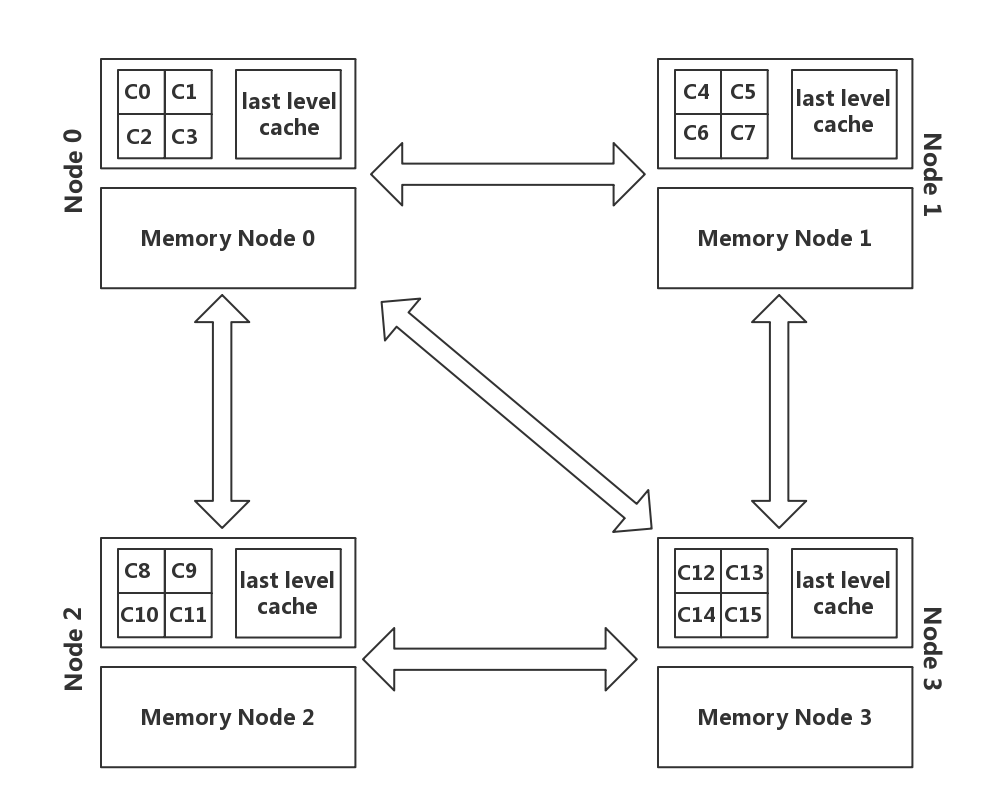
\includegraphics[width=5.0in]{NUMA.png}
	\caption{由四个四核处理器组成的NUMA系统}
	\label{Fig:numa}
\end{figure}
\section{NUMA架构及相关优化技术}

大型现代服务器通常由多个处理器节点组成,每个节点包含一个多核处理器和一块本地内存,其中本地内存上一般会有一个或多个内存控制器(memory controller)来处理来自本地节点或者其他节点上的核的内存访问请求,如图\ref{Fig:numa}所示。所有计算节点之间通过高速通信介质(interconnect)连接成单个缓存一致性系统,虽然物理内存被分割在了多个节点上,但是逻辑上物理地址空间仍然是全局共享的,也就是说所有核能够透明地访问所有节点上地物理内存。计算核心直接通过本地内存控制器来访问本地内存,而访问远程内存时则要通过节点间通信介质和远程内存的内存控制器。访问远程内存通常要比访问本地内存花费更多的时间,所以这些系统都具有非一致性内存访问延迟(Non-Uniform Memory access, NUMA)的特征。再考虑到内存和缓存的层级化(memory hierarchy)设计,访存的非一致性延迟特征更加显著。

显然要使应用程序在NUMA架构上获得更好的性能,在放置应用程序的线程和内存数据时必须考虑系统资源的物理构成和分布,比如为了充分利用访存操作的局部性,将线程及其访问的数据放置在同一个node上来避免远程内存访问的巨大开销。由于NUMA架构的服务器的广泛应用,目前很多操作系统都针对NUMA因素做了通用的优化,比如很多Linux系统都提供了numactl用于查看和优化NUMA系统中的线程放置和内存管理。使用numactl中的numastat用户可以查看各个NUMA节点的内存分配和节点之间的内存访问状况,比如查看每个节点上运行的进程在该节点和其他节点上各申请了多少内存。通过设置numactl的参数用户可以限定应用只能运行在某些特定NUMA节点集合上或者限定该应用的内存只能分配在某些NUMA节点集合上。除此以外,numactl还可以设置更为复杂的内存分配核管理策略,比如是否使用巨页(huge page),内存是否交织(interleave)分布在所有或者某些节点上。

上述操作系统提供的的这些优化工具一方面是非常粗粒度的,另一方面要求用户必须事先了解所运行的程序的特征,而现实的应用特征是复杂多变的而且事先难以预测的,所以仅靠这些通用工具很难最大化应用的性能,进一步的优化必须监测和考虑应用程序本身的特征。Carrefour\cite{dashti2013traffic}在分析了大量应用程序的访存特征后,认为应该根据应用的内存访问特征来使用合适的内存放置和管理策略,如图\ref{Fig:carrefour}所示,Carrefour支持三种内存访问策略:
\begin{itemize}
\item


复制(replication),即将同一个页的拷贝放置在多个NUMA节点上,复制将热点数据的访问压力分摊到了多个内存控制器,同时避免了远程内存访问,但是必须保持多个复制页内容一致,类似于缓存一致性,代价非常高昂,所以一般只对读写比很高的页采用复制策略;
\item  交织(interleaving),即将内存页平均放置在所有节点上,从而平衡各个内存控制器和节点间通信介质的访问压力,操作系统提供的交织是全局性的,而Carrefour中的交织可以只对部分页使用,进行更细力度的内存管理;
\item 协同放置(co-locate),即将共享内存页的线程与其共享的内存页放置在同一个节点上,从而减少远程内存访问和缓存的频繁刷新。
\end{itemize}

\begin{figure}[t]
	\centering
	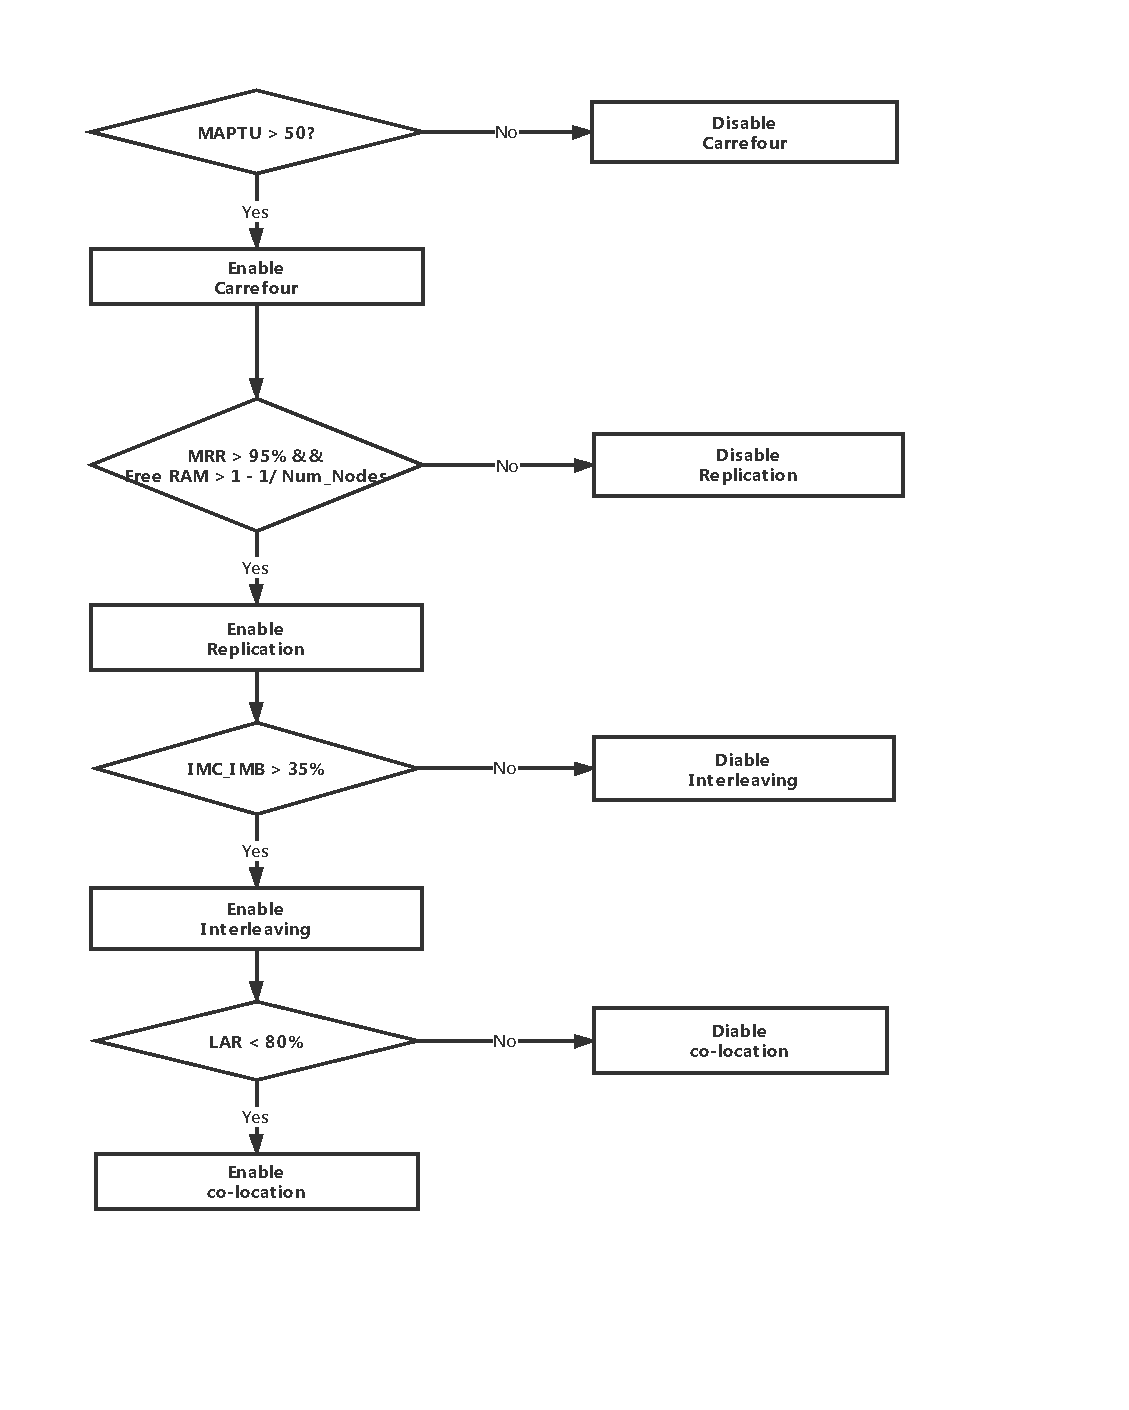
\includegraphics[width=4.2in]{Carrefour.pdf}
	\caption{Carrefour中的内存放置策略选择}
	\label{Fig:carrefour}
\end{figure}

虽然锁及其保护的数据在应用中的共享范围很广,但是这部分数据及其占比通常非常小,所以NUMA架构下的内存管理方面的优化对于锁的性能和其他方面的影响通常非常有限。而线程调度方面的优化对于锁的性能等方面的影响非常大,因为线程调度决定了锁的持有者和等待者的相对位置,影响锁的跨节点传递频率,进而影响到锁的性能,本章第三小节会对这点做详细说明。

\section{MCS锁与C-MCS锁}
尽管近年来事务性内存(transactional memory)\cite{larus2008transactional}开始流行,锁依然是保护多线程应用中共享数据完整性的一种最基本最主要的同步机制\cite{tallent2010analyzing}。线程对锁的竞争一直被认为是阻碍共享内存的多线程并行应用性能提升的关键因素,这是因为锁造成了并行程序中部分共享数据的串行访问\cite{tallent2010analyzing}。即使99\%的部分并行执行的应用也可能因为线程对锁的激烈竞争而导致性能下降甚至崩溃,所以使用锁的多线程应用程序的性能对于锁本身的性能尤其是锁在高度竞争情况下的性能越来越敏感\cite{johnson2010decoupling}。MCS锁由于其在性能、可扩展性和公平性等方面的良好表现被广泛应用于各种高性能系统中,而C-MCS锁是针对NUMA架构下内存及缓存访问的非一致性而对MCS锁做的适应性改进。本文研究的CAH线程放置框架针对的是基于队列的层级锁在锁的竞争变化的情况下难以同时兼顾锁的性能和长期公平性的问题,所以接下来我们以MCS锁和C-MCS为例对基于队列的层级锁的实现机制做详细介绍。
\subsection{MCS锁}
MCS锁是一种基于单向链表的高性能、可扩展、公平的自旋锁,由John Mellor-Crummey和Michael Scott在1991年提出, 其名称来源于发明人的名字首字母。

MCS锁中包含一个指向队尾的指针tail,每个竞争者在队列中用一个记录(record)表示,其中每个记录包含一个指向后继节点的指针和一个表示当前是否可以进入关键区域的布尔变量。如图\ref{Fig:MCS}所示,每个线程请求锁时将自己记录中布尔变量设为false,然后使用compare\_and\_swap这个原子操作来完成以下操作将自身的记录加入队列:1)使tail指针指向自己的记录;2)将自己的记录链接在前驱节点(如果有的话)的后面。如果该线程有前驱节点,则它在自身记录的布尔变量上自旋直到其被前驱节点设为true然后进入关键区域,否则该线程将自己的布尔变量设为true直接进入关键区域。放锁时只需要将后继节点的记录中的布尔变量设为true然后断开与后继节点的链接即可,如果没有后继节点则将tail设为null。
\begin{figure}[t]
	\centering
	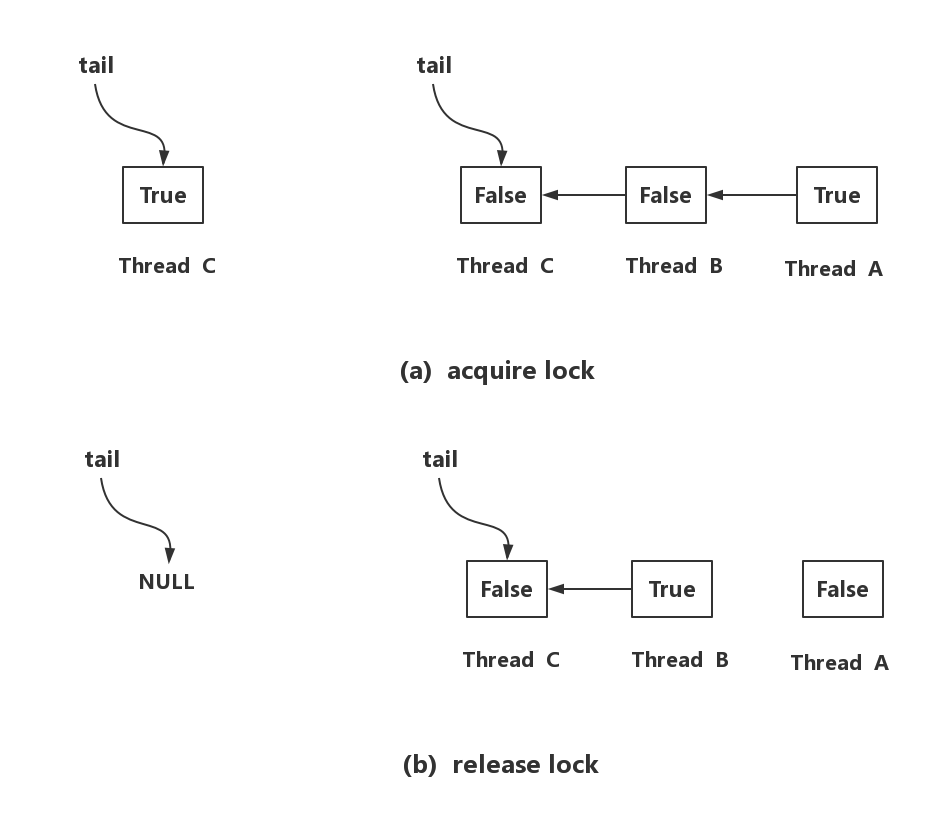
\includegraphics[width=5.6in]{MCS-lock.png}
	\caption{MCS锁拿放锁示例}
	\label{Fig:MCS}
\end{figure}

MCS的其正确性由算法本身和compare\_and\_swap这个原子操作共同保证。相比简单的spin lock,MCS通过显式存在的FIFO的队列保证了公平性,而每个线程只在本地标志变量上自旋并且只有自身和前驱节点对应的线程会访问该变量则保证了MCS锁的高性能和良好的可扩展性。

MCS锁的公平性和可扩展性是由其算法本身决定的,而其性能高低既与其实现算法有关,也与运行其的机器特征相关特征。由于锁保护的关键区域比较短,锁在线程间的传递时间可能比执行关键区域的时间还要长\cite{johnson2010decoupling},所以锁传递的效率(尤其是在高度竞争时)对于使用锁的并行应用的性能有很重要的影响。在NUMA架构的机器上,MCS为了维护其FIFO的公平性将不可避免地会产生大量的跨NUMA节点的锁传递,而跨NUMA节点的锁传递相比NUMA节点内锁传递的巨大代价会对其性能产生严重影响。

\subsection{C-MCS锁}
C-MCS锁是针对NUMA架构下内存及缓存访问的非一致性特征而对MCS锁做的适应性改进。它可以看作是一个两层的 MCS锁。如图\ref{Fig:CSTMCS}所示,该示例中展示了一个有9个线程的多线程应用,每个线程都差不多在同一个时刻竞争同一个锁(具体顺序如图(a)所示),其中线程T1到T5在节点0上而另外四个线程在节点1上,图a表示使用MCS锁时按照FIFO的顺序会有6次跨NUMA节点的锁传递(黄色表示跨节点锁传递),图b表示如果对锁的传递顺序加以合理调度则可以将跨节点的锁传递次数减为1,从而改善MCS锁在NUMA架构下的性能。通过a,b两图的对比可以看出C-MCS锁和MCS锁的本质区别,即C-MCS通过改变MCS锁的锁调度顺序,减少跨节点的锁传递频率,获得更好的性能。
\begin{figure}[t]
	\centering
	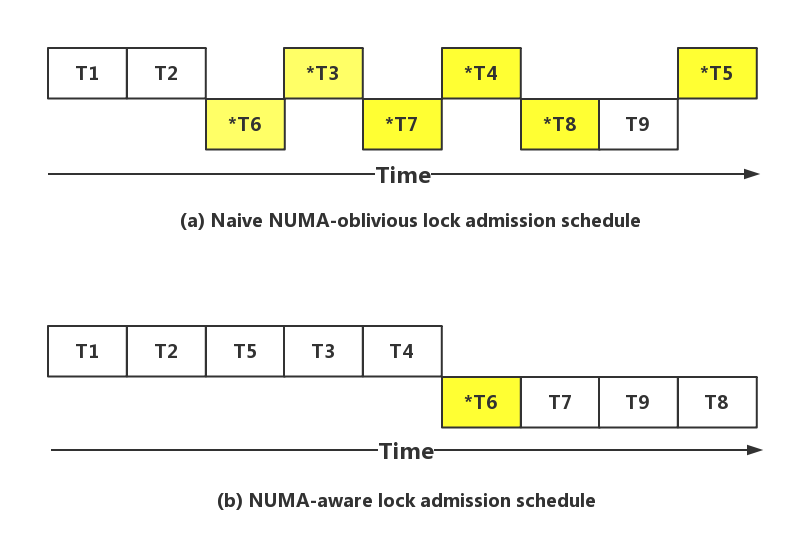
\includegraphics[width=5.0in]{CSTMCS.png}
	\caption{C-MCS锁的锁传递规则示例}
	\label{Fig:CSTMCS}
\end{figure}

C-MCS的具体实现还是以MCS锁为基础,包含一个全局MCS锁和每个节点上的一个局部MCS锁。全局MCS锁在所有节点之间共享,它的主要作用是将竞争分隔在各个节点内;而每个局部MCS锁只在其所在的节点内的线程间共享。一个线程只有同时拿到全局MCS锁和其所在节点的局部MCS锁才可以进入关键区域。每个要执行关键区域的线程先竞争本地MCS锁,每个节点上第一个拿到本地MCS锁的线程继续竞争全局MCS锁,其他线程直接从第一个线程继承全局MCS锁。执行完关键区域的线程先释放本地MCS锁,如果锁在本地节点的传递次数超过了预先设定的上限或者本地节点上没有其他请求者的时候才会释放全局锁。所以C-MCS锁的传递顺序可以描述为,锁的持有者将其传给一个本地的最早请求者当且仅当以下两个条件同时满足:
\begin{itemize}
\item  本地节点当前至少有一个请求者;
\item  其所在本地节点的锁传递次数还未超过预先设定的threshold;
\end{itemize}
其中设置threshold是为了防止深层的不公平。

C-MCS锁在决定锁的调度顺序时考虑了等待队列中的线程和当前拿锁线程在NUMA拓扑上的相对位置,从而减少了锁在NUMA节点之间的迁移频率,提高锁的总吞吐率。相反的,标准的MCS锁不能感知底层的NUMA因素,所以只能按照线程的到达时间即线程请求锁的时间来决定锁的传递顺序,所以在NUMA架构上会有性能损失,C-MCS锁放弃了MCS锁全局FIOF的锁传递顺序,只保证单个节点内的FIFO锁传递顺序,所以其高吞吐率的获取是以牺牲一定的短期公平性(改变锁的传递顺序)为代价的。

我们下一章将通过实验和分析说明如果线程放置不当,C-MCS锁在牺牲MCS锁短期公平性的同时也可能会带来长期公平性方面的损失。

\section{线程调度与放置}

线程调度/放置对于NUMA架构下锁集中的应用的的性能有非常重要的影响\cite{pusukuri2014shuffling},这是因为线程调度/放置决定了线程在NUMA节点上的分布,而线程在NUMA节点上的分布影响跨NUMA节点的锁传递比例进而影响锁及应用的性能。本小节中我们先介绍NUMA架构下通用的Linux调度器的线程调度策略,然后介绍NUMA架构下针对锁的线程调度/放置策略的优化,最后介绍层级锁中的现有的几种线程放置策略。
\subsection{NUMA架构下Linux线程调度}
作为资源管理的核心部分,操作系统的线程调度器的主要职责是保证准备好的线程被调度到可用的核上去。在Linux系统当前使用的调度算法CFS(Completely Fair Scheduling)\cite{lozi2016linux}是WFQ(Weighted Fair Queueing)调度算法的一种实现。在单CPU系统中,CFS的实现非常简单。为了实现公平调度,CFS定义了一个固定长度的时间间隔,在该间隔内系统中的每个线程至少运行一次,该间隔被按照线程的权重按比例分为若干个大小不一的时间片(time slice),每个线程的权重就是它的优先级。正在运行的线程会不断增加它的已运行时间(vruntime),当它的vruntime超过分配给其的时间片时,如果当前有其他可以运行的线程,那么正在运行的线程就会被抢占;另外当前运行的线程也可能被另一个被唤醒的vruntime更小的线程抢占。具体的实现中,线程被组织为一个用红黑树实现的运行队列(runqueue),如图\ref{Fig:CFS}所示,在该运行队列中,每个线程按照其vruntime排序,当CPU需要找一个线程来运行的时候,红黑树中最左边的线程也就是vruntime最小的线程会被选择。

\begin{figure}[t]
	\centering
	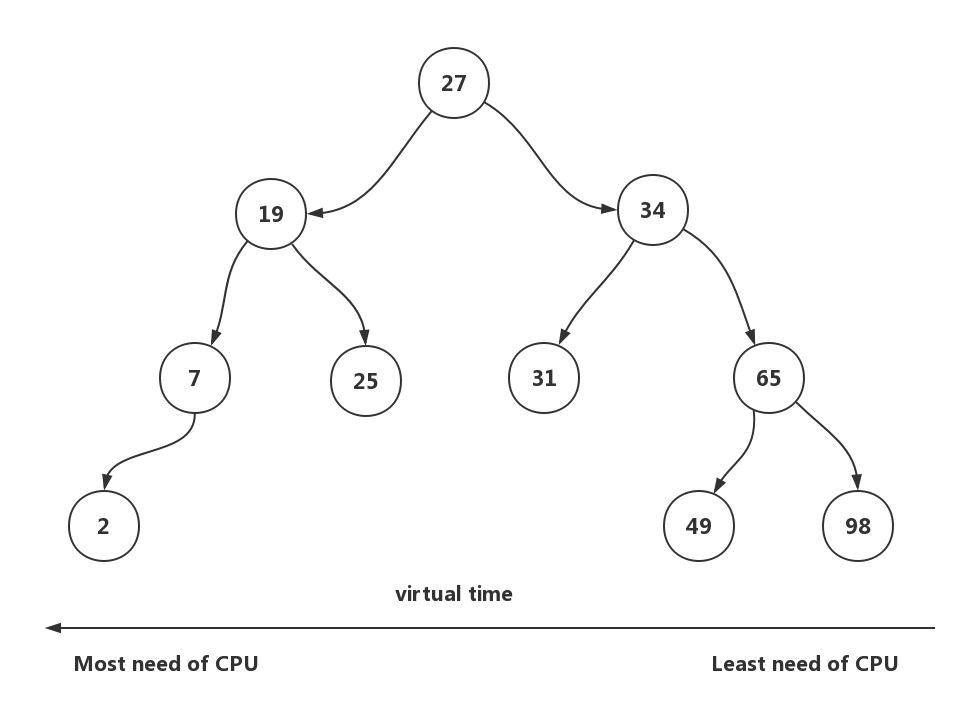
\includegraphics[width=5.0in]{CFS.png}
	\caption{CFS示例}
	\label{Fig:CFS}
\end{figure}

在NUMA架构下,由于内存访问非一致性等原因的存在使得CFS的实现变得非常复杂。为了保持良好的可扩展性,CFS使用了per-core runqueue,即每个核一个运行队列,这样设计的主要原因是进程切换(context switch)发生在关键路径上而每个核一个运行队列使得进程切换时只需要访问本地运行队列。但是为了使调度算法在使用了per-core runqueue时能够正确高效地运行,必须有额外的机制来保持运行队列的负载均衡。Linux CFS采用的方法是周期性地运行一个负载均衡算法来保持所有队列负载的大致均衡,具体实现中采用了层级化的策略(hierarchy strategy),所有核被逻辑上组织为一个层次结构,该层次结构的最底部是单个核,这些核在下一层及后面的层被如何分组是由它们对物理资源(内存,各级缓存)的共享拓扑决定的。每层的结构被称为一个调度域(scheduling domain),负载均衡算法按照自下而上的顺序在每个层次的调度域内运行。将所有核组织成一个层次结构然后自下而上运行负载均衡算法相比直接在所有核之间通过线程迁移来调节负载的主要优势在于可以减少跨深层NUMA因素的线程迁移比例从而使得负载均衡算法的开销尽可能的小,这与层级锁的设计思路很相似。

现代操作系统的调度器在做线程调度时主要考虑因素有三点:1)通过线程在核之间的迁移来保证可运行的线程能被调度到可用的核上去;2)保证核之间负载的大致均衡;3)在NUMA架构下使负载均衡算法的代价尽可能大地小。这种调度算法非常适合相互之间没有关系的线程即不通过共享内存通信的线程,它能够避免线程之间对于节点层次的共享资源例如缓存、内存通道等的使用发生冲突(缓存失效等),它的前提假设是线程之间的通信非常少并且远不如节点层次的本地资源使用冲突重要。但是在锁集中并且存在大量线程间共享数据的多线程应用中,显然线程之间的通信是居于主导地位的,保证线程之间通信的高效的重要性要高过线程对资源的独享重要性\cite{dice2015lock},所以操作系统通用的调度器不能很好的满足这类场景的需求。另外考虑到层级锁中通过挖掘线程之间的亲和性来做锁调度,而通用的调度器将相关的线程分散在所有节点的可用核上使得层级锁可以挖掘的线程间的亲和性非常有限。

总的来看,通用的调度器并不适合NUMA架构下锁集中的多线程应用尤其是使用层级锁的多线程的应用,为了使这些应用获得更好的性能,必须有定制化的考虑应用具体特征的线程调度/放置方法,也就是说应该使用定制化的调度器或者让应用程序来做自身的线程调度/放置。


\subsection{NUMA架构下针对锁的线程调度优化}
在NUMA架构下,操作系统的通用调度器很容易造成锁在NUMA节点之间的频繁迁移进而导致其性能下降,所以出现了很多定制化的线程放置/迁移策略,比如最朴素的做法是将请求锁的线程迁移到当前持锁的线程所在的节点\cite{sridharan2006thread},即将线程迁移到包含锁及其保护的数据的缓存的节点上而不是相反,然而这种简单的迁移存在两个问题:1)线程迁移次数不可控;2)容易导致负载不均衡,最终的结果可能是得不偿失。shuffling\cite{pusukuri2014shuffling}是一种能够兼顾负载均衡和迁移代价的适合锁集中的应用的线程放置/迁移策略。shuffling通过将到达时间(lock arrival time)差不多的线程放置在相同的节点上来避免锁在节点间随意迁移,具体做法如图\ref{algo:shuffling}所示,shuffling周期性地收集各个线程的到达时间;然后按照到达时间将所有线程排序分组,到达时间相似的线程被分到相同的组里,每组的大小等于每个节点上的计算核心数;最后通过迁移某些线程将分好的每个线程组映射到NUMA节点上去。相比简单的线程迁移,shuffling保证了负载均衡并且可以很好地控制线程的迁移。

\begin{algorithm}
% \begin{algorithm}[H] % 强制定位
\caption{Shuffling框架}
\label{algo:shuffling}
\begin{algorithmic}[1] %每行显示行号
\Require N:Number of threads, C:Number of Nodes % 输入
\Repeat
\State {\bf Monitor Threads} -- sample lock times of N threads
\If{\emph{lock times exceed threshold}}
    \State {\bf Form Thread Groups} -- sort threads according to lock times and divide them 
    into C groups
    \State {\bf Perform Shuffling} -- shuffle threads to establish newly computed thread groups
\EndIf
\Until{application terminates}
\end{algorithmic}
\end{algorithm}

Shuffling适用于使用传统锁的锁集中的应用,它与层级锁是两种针对NUMA架构的访存非一致性特征的不同的锁改进方案,shuffling通过将连续请求锁的线程调度到相同的NUMA节点上来降低访存非一致性对锁性能的影响,而层级锁是通过NUMA感知的锁调度来降低访存非一致性的影响的。

\subsection{层级锁中现有线程调度策略}
层级锁一般应用于运行在NUMA架构上锁集中的高性能应用中,在这种场景中锁的性能在很大程度上决定了应用整体的性能,层级锁通过感知线程在NUMA节点上的相对位置调度锁来降低NUMA因素对锁性能及应用整体性能的影响。由于层级锁高性能的发挥依赖于线程在NUMA节点上的分布,所以线程调度/放置策略对锁的性能有很重要的影响\cite{guiroux2016multicore}。层级锁中现有的线程放置策略主有以下三种:自由调度(Free-Range),紧凑放置(Compact)和平均放置(Even)。

自由调度,即操作系统调度器的默认线程调度策略。应用程序对于线程的放置没有任何限制,线程的迁移调度全部交给操作系统的调度器来完成。如上节所述,NUMA架构下的Linux CFS调度器充分考虑了各个节点和核上的负载均衡,保证了可运行的线程能被及时调度到可用的核上去,能够通过激进的线程迁移来达到更好负载均衡和其他调度目标\cite{guiroux2016multicore}。但是对于层级锁来说,由于默认的调度器并不知道线程和应用程序的所属关系,也不知道线程之间的锁竞争关系,简单的负载均衡很容易将同一个应用的线程分散到多个节点上去从而减少层级锁所能挖掘利用的局部性进而造成锁性能的极大损失。此外,在竞争线程较多时自由调度也可能带来锁的持有者被抢占或者等待者被抢占等问题,从而导致性能方面的严重损失。

紧凑放置,由于层级锁偏向于寻找最近的等待者完成锁传递,因此最自然的线程放置策略是将线程尽可能地放得紧凑,这也是目前大多数层级锁(HMCS锁\cite{chabbi2015high}, HMCS-T锁\cite{chabbi2017efficient}, CST 锁\cite{kashyap2017scalable})中的默认线程放置策略。具体来说,新的线程会尽可能地被放置在当前NUMA节点的某个可用计算核心上,只有当前的NUMA节点上没有可用的计算核心时,新的线程才会被放置到一个新NUMA节点的某个专用计算核心上。相比自由调度,紧凑策略更好地控制了CPU资源的分配,将每个线程绑定到一个专用的核上也能避免线程抢占带来的问题。此外,它限制了线程分布到的节点数,使得锁的持有者在释放锁时有更大概率找到一个本地等待者,从而降低锁的跨节点传递频率,改善锁的性能。但是紧凑放置在大多数情况下不可避免地会导致线程在NUMA节点之间分布的不均匀,再加上层级锁锁传递策略的本地偏好的特性,使得其难以保证层级锁的长期公平性(long-term fairness),即从长远来看总的吞吐率确实很高,但是单个线程的吞吐率之间差异很大。

平均放置,AHMCS\cite{chabbi2016contention}锁中,作者为了说明AHMCS能够快速适应锁的竞争强度的变化将线程平均放置在所有NUMA节点上。由于每个节点上运行相同数量的线程,所以每个节点具有相同的将锁保持在其上的能力,因此平均放置理论上能够很好地保证层级锁的长期公平性。但是相比紧凑放置,在锁的竞争不是很激烈时每个节点都不可能将锁长期保持在其上,所以很容易导致锁在节点间的频繁迁移,使得层级锁不能有效地发挥其性能优势,进而造成性能损失。


自由调度是Linux系统通用的调度策略,其在线程调度时主要考虑的是负载均衡和和CPU在线程间的公平共享,并没有考虑也不能感知到线程对锁的竞争关系,所以不能使层级锁充分发挥其在NUMA架构上的性能优势;紧凑放置使得层级锁能够尽可能地挖掘线程之间的局部性,减少锁的跨节点传递,提高性能,但是紧凑放置结合层级锁的锁传递算法容易带来长期不公平问题;平均放置理论上能够保证层级锁的长期公平性,但是它相比紧凑放置容易导致性能损失。现有的线程放置策略或者不能同时保证层级锁的高性能和长期公平性,或者只能在锁的竞争强度足够高的情况下保证层级锁的高性能和长期公平性,而公有云等现实应用场景中一方面对这两方面都有很高的要求,另一方面这些应用中锁的竞争随着需求的变化是否复杂多变并且难以预测的\cite{chabbi2016contention}\cite{johnson2010decoupling},为了满足这些场景的需求,我们需要一种能够适应竞争变化并且能够同时保证层级锁的高吞吐率和长期公平性的新的线程调度/放置策略。

\section{本章小结}
本章主要对NUMA架构的访存非一致性特性、基于队列的层级锁考虑NUMA因素下对传统基于队列的锁所做的优化,线程调度与放置技术及其对基于队列的层级锁的性能和长期公平性的影响等做了详细说明。基于队列的层级锁通过NUMA感知的锁调度改善了队列锁在NUMA架构下性能,而NUMA感知的锁调度使得线程在NUMA节点上的分布会影响到基于队列的层级锁中的锁传递顺序,所以如果线程在NUMA节点上的分布不当也可能会影响到基于队列的层级锁的性能和长期公平性。下一章我们将会通过对实验和分析来说明线程放置对基于队列的层级锁的性能和长期公平性的影响。